%*-----------ORIENTADOR -------------------------------------------------------------
\begin{frame}[t]{Horta-bot}
    \transboxout[duration=0.5]
    \framesubtitle{Marco Reis}
    \begin{columns}
        \column{.075\textwidth}
        \column{.4\textwidth}
            
            \begin{figure}
                \vspace*{-0.75cm}
                \hspace*{-1.5cm}
                %
\includegraphics[width=.8\textwidth]{marcoreis.png}
                \roundpic[xshift=0cm,yshift=0cm]{6cm}{5cm}{marcoreis.png}
            \end{figure}
            
        \column{.55\textwidth}
                %\justifying
                %// Senior Engineer and Researcher with more than 20 years of experience in industrial project management and R&D, including the implementation of two automobile plants in Brazil as well as in steel making, power generation and automation. Develops robotic and manipulator tool designs, autonomous vehicles, asset management, RCM, TPM, reliability and maintenance of critical equipment, and evaluation in FMEA application. In recent 10 years he has worked in development robotic projects.
                \vspace*{0.1cm}
                \justifying
                
                Engenheiro e Investigador sênior com mais de 20 anos de experiência em gestão de projetos industriais e P\&D. Nos últimos 10 anos tem trabalhado no desenvolvimento de projetos robóticos, tais como, veículos autônomos, ferramentas robotizadas e manipuladoras
        \column{.045\textwidth}
    \end{columns}
 %*----------- notes
    \note[item]{Notes can help you to remember important information. Turn on the notes option.}
\end{frame}
%-

%*----------- SLIDE -------------------------------------------------------------
\begin{frame}[t]{Justificativa} 
    \transdissolve[duration=0.5]
    \newcommand\vertspacejust{0.12cm}
    %\newline
        \begin{columns}[t]
            \column{.05\linewidth}
            \column{.6\linewidth}
                    \justifying
                    A busca por alimentos orgânicos tem crescido  \cite{sebrae:organicos} \cite{PesquisaOrganicos:online}. \\ \vspace*{\vertspacejust}
                    O cultivo de pequenos temperos e hortaliças no ambiente domiciliar favorece uma cultura mais "verde" e participativa \cite{G1:pequenoagricultor} \\ \vspace*{\vertspacejust}
                    A rotina da vida urbana torna o tempo um recurso escasso, dificultando atividades de cultivo \cite{G1:3xtransito} \\ \vspace*{\vertspacejust}
                    Há uma longa e complexa cadeia logística na disponibilização de alimentos orgânicos \cite{silva:cadeiaprodutiva}  \\ \vspace*{\vertspacejust}
            \column{.45\linewidth}
            
            \begin{center}
            %\centerline{
                \begin{figure}
                    \vspace{-1cm}
                    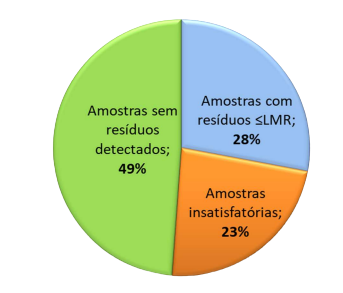
\includegraphics[width=0.85\textwidth]{anvisa-2018-irregularidades.png}
                    \caption{\centering Resultados do monitoramento de agrotóxicos nos alimentos \cite{ANVISA-PARA:online}}
                    % \hspace{125pt}
                    % \roundpic[xshift=0cm,yshift=0cm]{4cm}{5cm}{}
                    %\caption{Pista de corrida \cite{agostini2007}}
                \end{figure}
            %}
            \end{center}
        \end{columns}
%*----------- notes
    \note[item]{Notes can help you to remember important information. Turn on the notes option.}
\end{frame}
%-

%*----------- SLIDE -------------------------------------------------------------
\begin{frame}
    %\transdissolve[duration=0.5]
    %\hspace*{-1cm}
    \begin{columns}
        %\column{.01\textwidth}
        \column{0.4\textwidth}
            ~\hfill
            \vbox{}\vskip-1.4ex%
            \begin{beamercolorbox}[sep=6em, colsep*=18pt, center, wd=\textwidth, ht=\paperheight]{title page header}%
                \begin{center}
                    \textbf{\huge{PROBLEMA}}\par
                    \vspace*{0.3cm}
                    \textbf{\huge{DE}}\par
                    \vspace*{0.3cm}
                    \textbf{\huge{PESQUISA}}
                \end{center}
            \end{beamercolorbox}%
        \hfill\hfill
        \column{.05\textwidth} 
        \column{.55\textwidth}
        \begin{center}
            \huge{\textbf{"De que forma é possível cultivar hortaliças orgânicas de maneira autônoma no ambiente residencial dos centros urbanos?"}}
        \end{center}
        \hfill
       
    \end{columns}
  
 %*----------- notes__
    \note[item]{Notes can help you to remember important information. Turn on the notes option.}
\end{frame}
%-

%*----------- OBJETIVO GERAL -------------------------------------------------------------
\begin{frame}[c]{Objetivo Geral} 
    \transdissolve[duration=0.5]
   
    \begin{center}
        \Wider{%
        \begin{shaded}
        \begin{center}
            \vspace*{0.4cm}
            \resizebox{!}{1.3cm}{%
               % \color{bg} O objetivo é ter um objetivo.
                \begin{tabular}{ccc}
                    \textbf{Desenvolver um sistema robótico capaz} \\ 
                    \textbf{de realizar o plantio e monitoramento} \\ 
                    \textbf{de hortaliças}       
                  \end{tabular}
            }%
        \end{center}
        \end{shaded}
        }%
    \end{center}
    
   
%*----------- notes
    \note[item]{Notes can help you to remember important information. Turn on the notes option.}
\end{frame}
%-
%*----------- SLIDE -------------------------------------------------------------
\begin{frame}[t]{Objetivos Específicos}
    \newcommand\vertspaceobjesp{0.12cm}
    \transboxout[duration=0.5]
    \begin{columns}
        \column{.1\textwidth}
        \vspace*{1cm}
        \hspace*{3cm}
        \column{1.8\textwidth}
                \Large{
                \\ \vspace*{\vertspaceobjesp}
                Analisar as técnicas e os requisitos para conceito do projeto\\ \vspace*{\vertspaceobjesp}
                Implementar algoritmos de monitoramento            \\ \vspace*{\vertspaceobjesp}
                Analisar resultados dos testes físicos e simulados \\ \vspace*{\vertspaceobjesp}
                Validar o conceito}
    \end{columns}
 %*----------- notes
    \note[item]{Notes can help you to remember important information. Turn on the notes option.}
\end{frame}
%-